\chapter{pEPR Spectroscopy of Densely Packed Nitroxide Radicals}

\section{Coherent Spin Motion under Pulsed Microwave Field}
When a spin system is excited with a microwave pulse, its evolution is described with the set of equations that is known as the Bloch equations.
\subsection{Bloch Equations}
\subsection{Spin Relaxation Times}
\subsection{Spin Packets}

\section{Instrumentation}
\subsection{Pulse Sequences and Measurement Techniques}
\subsubsection{The Refocused Spin Echo}
The Hahn Echo sequence consists of two pulses, the $\pi/2$ pulse and the $\pi$ pulse, separated in time by $\tau$: $\pi/2 - \tau - \pi - \tau - echo$. Initially, the macroscopic magnetization of the spin system is aligned along $\vec{B_0}$: $\vec{M}_0=M_Z~\vec{e_Z}$. The $\pi/2$ microwave pulse has such length $t_{\pi/2}$ and amplitude $B_1$ that, during the pulse, $\vec{M}$ nutates to the $xy$ plane, where it keeps precessing about $\vec{e_Z}$ after the end of the pulse. The difference in local environments for each individual spins in the spin packet, as well as the interactions between the spins, that make up $\vec{M}$, leads to slightly different precession frequencies $\omega_L^i$ of the spins. After some time $\tau$, the difference in the precession frequencies translates into the differences in phases so that the vector sum of the excited spins averages down to $\vec{0}$ for sufficiently long $\tau$. In other words, the excited spin packet dephases with time. The dephasing due to different local spin environments can be reversible if the deviations of the precession frequencies do not depend on time, as is the case for separated electrons in an inhomogeneous solid. In such case, a $\pi$ pulse can be applied to the spin system to flip every single spin in the dephased spin packet by 180$\deg$ in a plane containing $\vec{e}_Z$, so that the spins keep precessing in the $xy$ plane, but the direction of precession is inverted for them, leading to the effect that is opposite to the initial dephasing. So a $\tau$ after the $\pi$ pulse excites the spin packet, the accumulated phase differences become the smallest and the packet recovers its macroscopic magnetization $\vec{M}$ that oscillates in the $xy$ plane with $\langle\omega_L^i\rangle$ and can be detected. The recovered $\vec{M}$ at $t=\tau$ after the $\pi$ pulse is called the refocused spin echo. The difference in $\omega_L^i$ leads to a further dephasing of the considered spin packet and to the vanishing of $\vec{M}$.\\
\subsubsection{Spin Echo Decay and Phase Memory Time}
\subsubsection{Inversion Recovery and Spin-Lattice Relaxation Time}

\subsection{Broad-Band Excitation and Instantaneous Diffusion}
In Section /// it is shown that in a densely packed radical system, as in a TEMPO-Salen cathode film, the phase memory time can be shorter than $T_m\leq100$~ns. That is, the spin echo is decaying by $e\approx3$ at $t=100$~ns. The short phase memory time limits the duration of the pulse sequence at which the echo is detectable. For a $\pi/2-\tau-\pi-\tau-echo$ sequence, with a hardware limitation on $\tau\geq t_d\approx100$~ns, the pulse sequence is longer than $t>200$~ns. By this time, the spin echo decreases by $e^2\approx7$ and may be comparable to noise. The limitations imposed by the finite $T_m$ and $t_d$ force one to use shorter microwave pulses. 
\par
A short microwave pulse may have a spectral width comparable to the width of the observed spectrum. According to the Fourier theorem, the spectral width of a pulse is inversely proportional to the pulse length: $\Delta\omega\sim 1/t_p$. A spectrum of a 100~ns long rectangular pulse shown in Figure /// is ///MHz wide (FWHM). 

\begin{figure}[h]
\center
	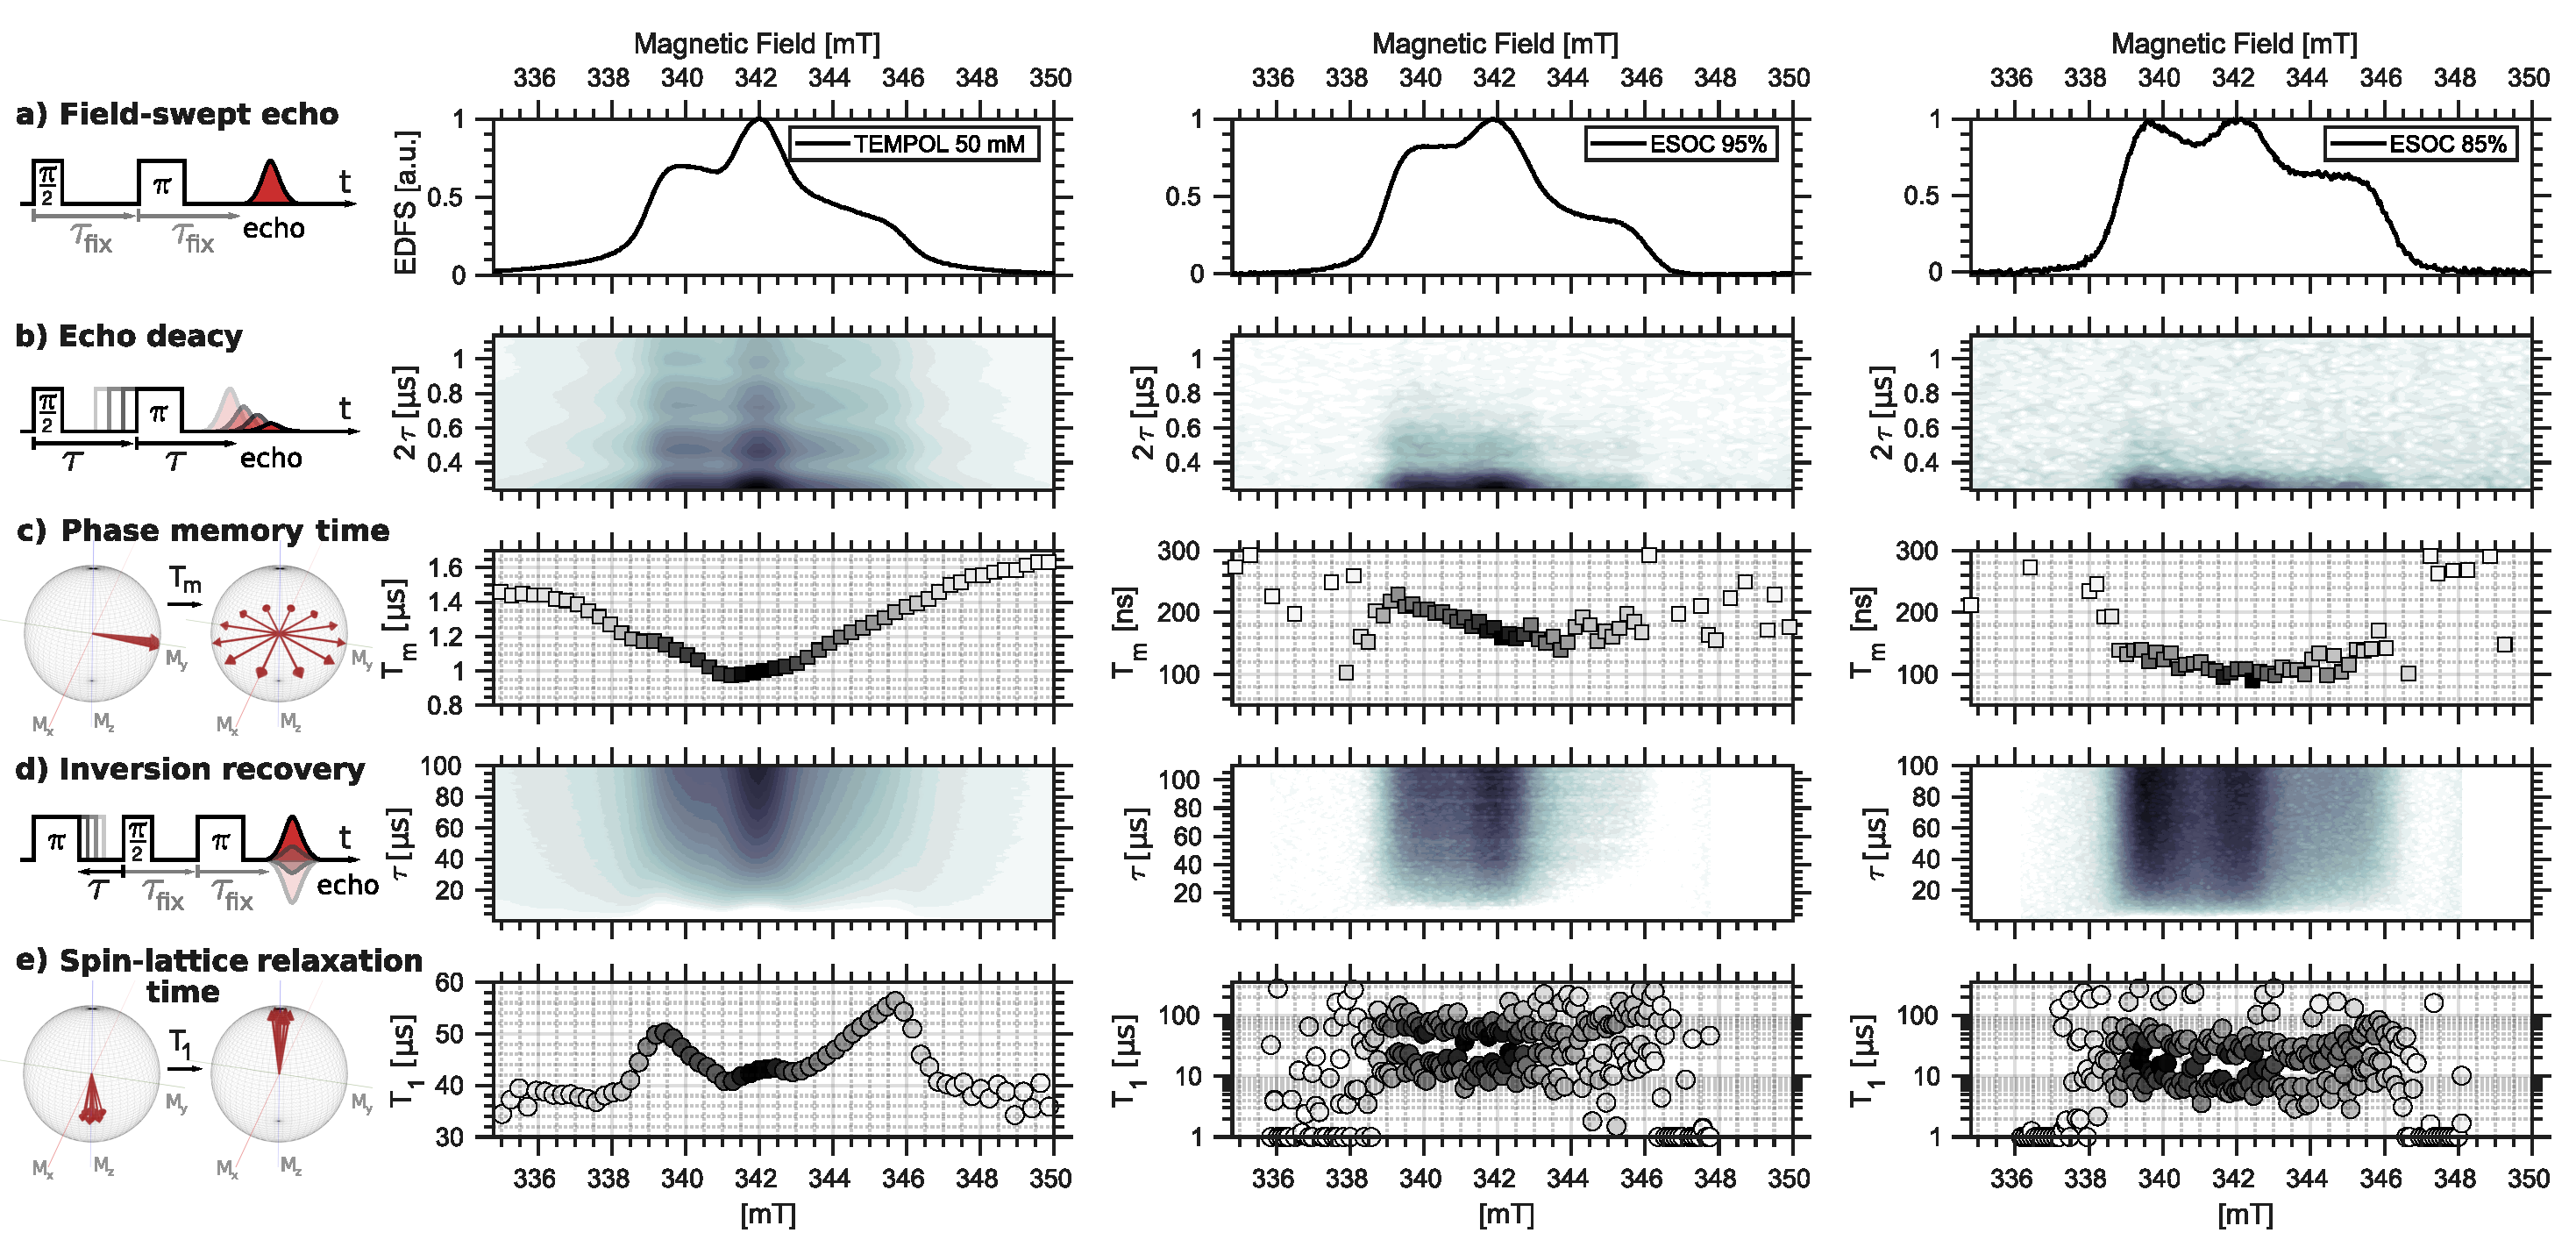
\includegraphics[width=1\textwidth]{./pulse/figures/FSE_DTBS_FSE_RELAX_T1Tm.pdf}
	\caption{XXX}
	\label{fig:spectra_of_pulses}
\end{figure}


\section{Pulsed EPR Spectroscopy of a charged pDiTBuS Cathode film}

\subsection{Field Swept Echo of a charged pDiTBuS Cathode film}
\begin{figure}[h]
\center
	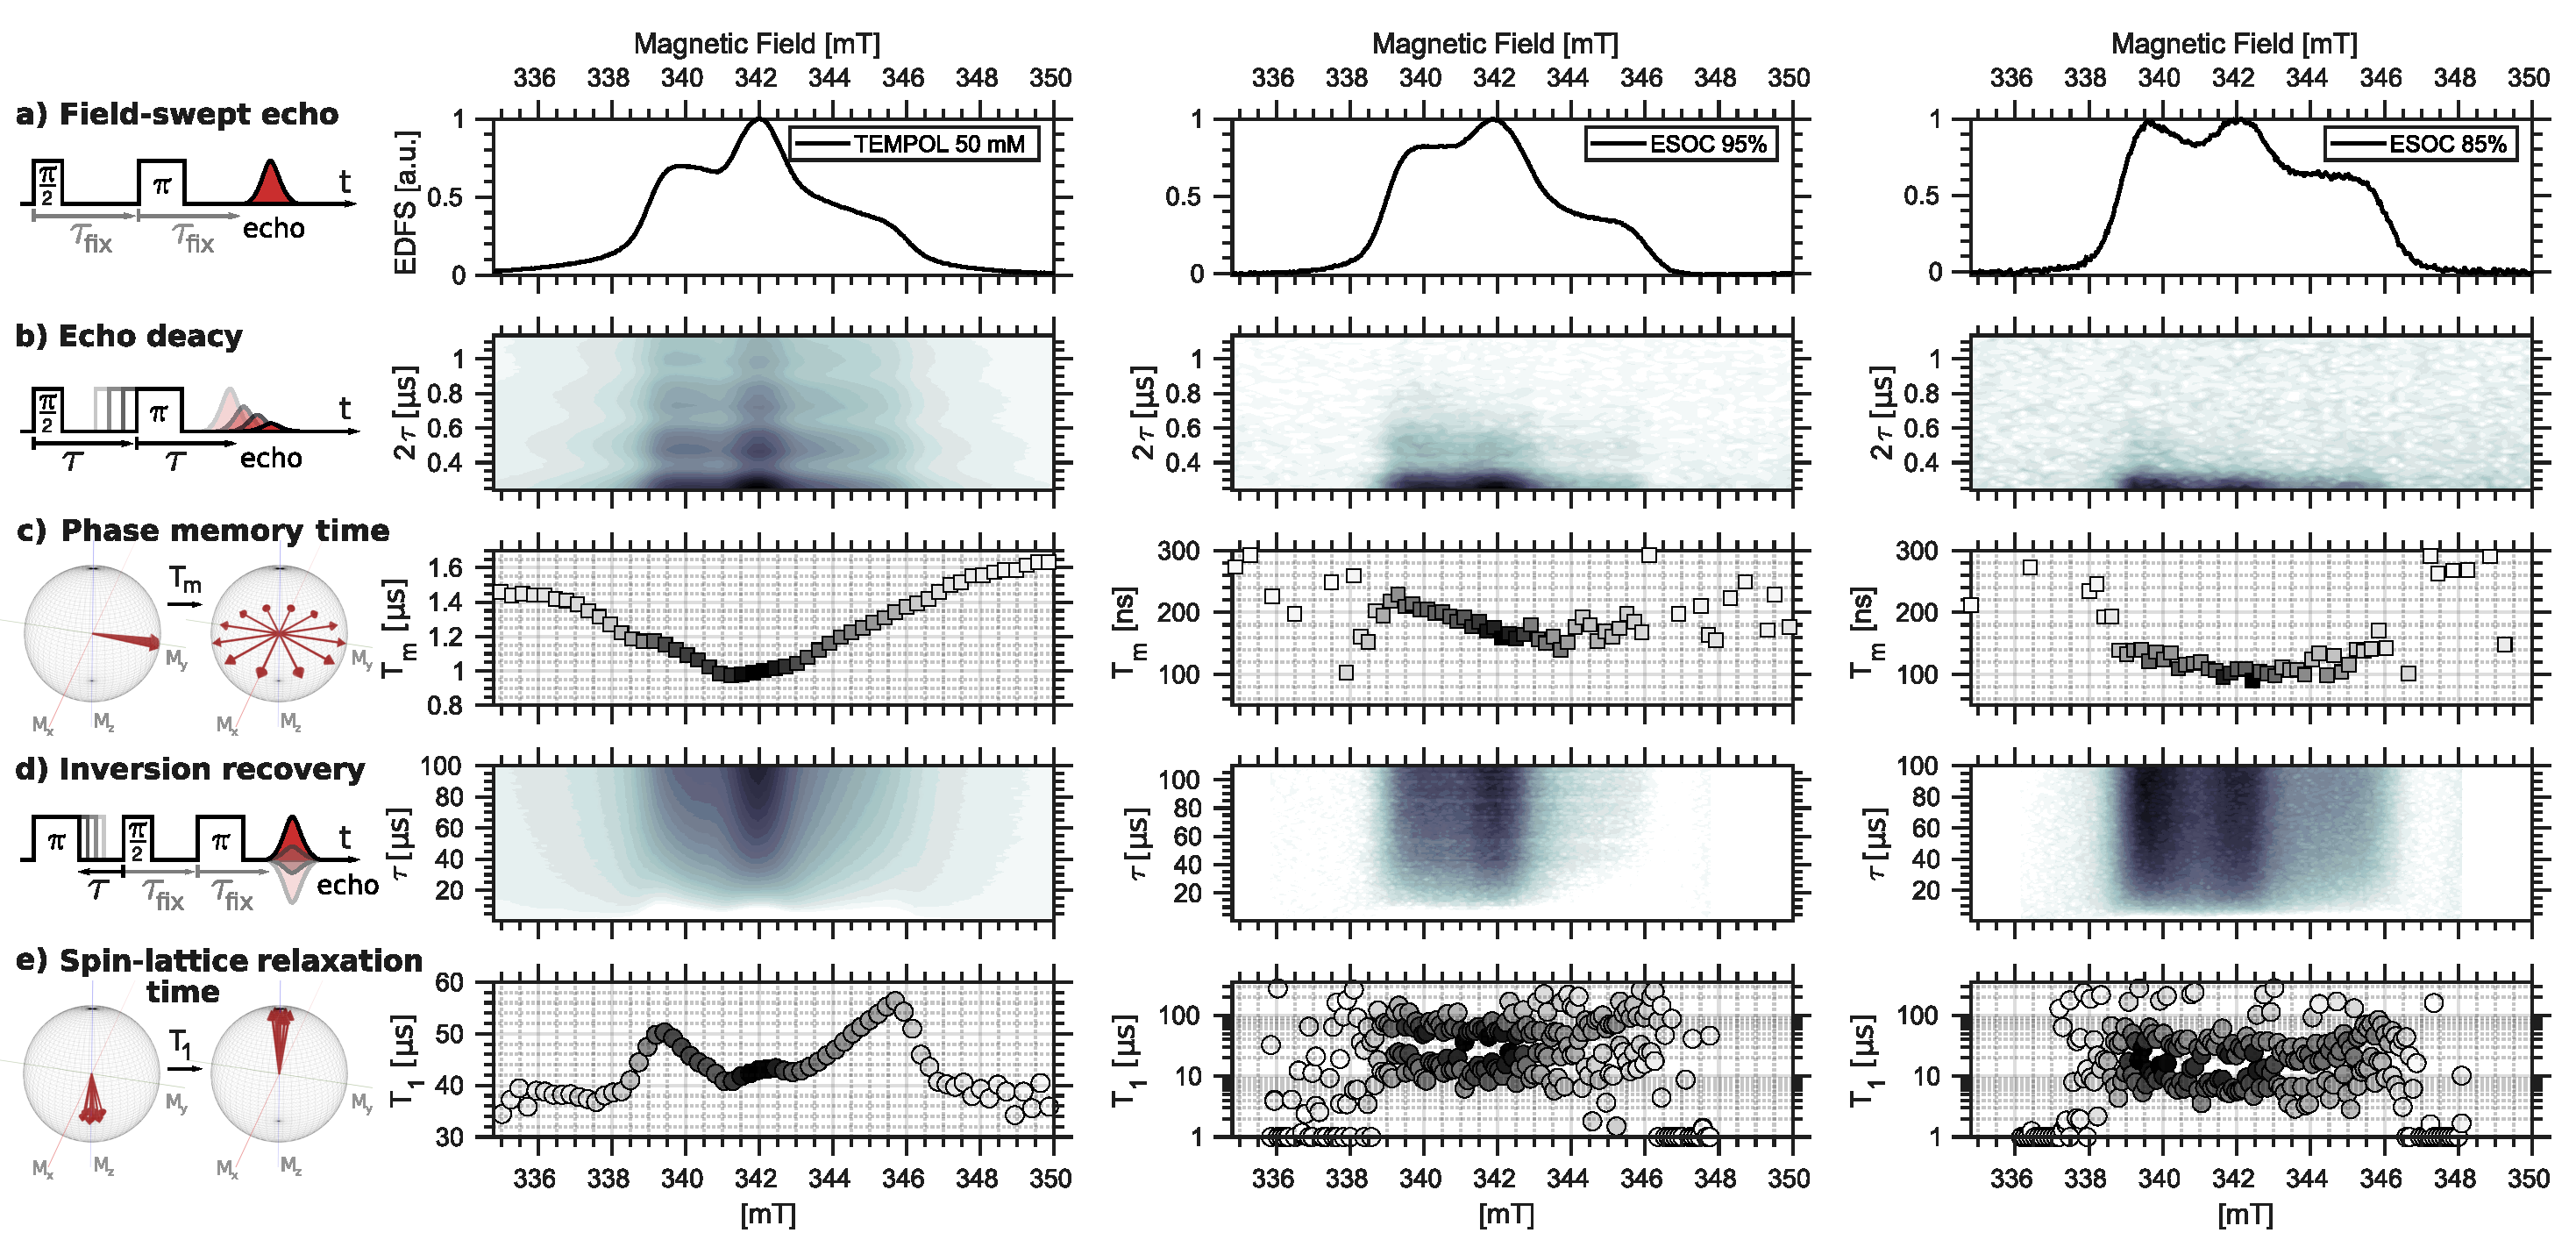
\includegraphics[width=1\textwidth]{./pulse/figures/FSE_DTBS_FSE_RELAX_T1Tm.pdf}
	\caption{XXX}
	\label{fig:Figure_FSE1}
\end{figure}


\subsection{Estimation of Local Spin Concentrations with Instantaneous Diffusion}
\subsection{Spin Relaxation in a charged pDiTBuS Cathode Film}
\subsection{Pade-Laplace Deconvolution of Echo Decay Transients}

\subsection{Detection of Domains with Poor Conductivity}
\label{domains_distinction_by_relaxation}

\subsection{Towards Imaging of Spin Concentration in Battery Electrodes}
One can obtain a spatially resolved image of the spin concentrations inside a battery electrode by encoding the position with a gradient of the magnetic field. With the procedure described in Section~\ref{domains_distinction_by_relaxation} and using a pair of electromagnetic coils to superimpose a gradient of $B_0$ one can not only measure the spin concentrations that are present in the electrode, but also to locate the electrochemically inactive domains and to visualize the conductive paths throughout the electrode.

\subsection{Unusual Peak Ratios in a Highly Charged Cathode Film}




